\section{Communication Serveur/GUI}

\subsection{Présentation}

\par La communication entre le serveur de l'application et les conteneurs repose sur une connexion SSH. L'application se connecte au serveur contenant les dockers afin de communiquer les messages et d'exécuter les commandes qui lui sont donnés.

\par L'utilisation de Symfony a permis l'utilisation de la librairie libssh2 de PHP. Cette librairie permet de gérer facilement une connexion SSH en PHP.

\subsection{Processus de communication}

\par Le processus de communication repose sur un système de questions/réponses. Le client demande des informations et le serveur lui répond.

\begin{figure}[H]
\centering
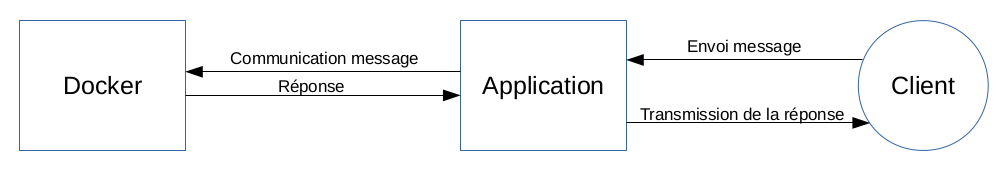
\includegraphics[width=0.8\textwidth]{./img/communication/com.png}
\caption{Communication entre le client et le conteneur Docker}
\end{figure}


\subsubsection{Première requête envoyée (clic sur le bouton Lancer)}

\par L'application reçoit la requête du client. Elle va créer la commande qui permet de démarrer un conteneur docker et de lancer le script qui se charge de la compilation et de l'exécution du programme. La commande est ensuite passé au service GestionSSH qui se charge de se connecter en SSH au serveur qui contient les conteneurs et d'exécuter la commande grâce à un shell. 

\par L'application récupère ensuite la sortie standard du programme, toujours grâce au service GestionSSH. Elle répond ensuite au client qui attend toujours la réponse du serveur. Le client affiche ensuite la réponse dans la vue JQConsole.

\subsubsection{Envoi des requêtes suivantes}

\par Dans certains programmes, l'utilisateur a besoin de répondre au programme pour que celui-ci se termine (fonction d'inputs). Dans ce cas, l'application teste si le docker est encore ouvert et le redémarre si oui. Le message est ensuite passé au service de GestionSSH qui se charge de le transmettre au conteneur grâce à SSH.

\par L'application récupère de nouveau la sortie standard du programme pour l'envoyer au client. Cette opération se répète jusqu'à ce que l'exécution du programme soit terminée.

\subsection{Problème de la communication}

\par Le principal problème apparu lors du développement de la communication est dû à la non persistance des objets en PHP. En effet, à la fin de chaque requête, PHP supprime tous les objets qui ont été créés pendant la requête. Il nous était donc impossible de garder une connexion SSH ouverte pendant toute l'exécution du programme. Après de nombreuses recherches, nous avons décidé de créer une nouvelle connexion SSH à chaque nouvelle requête. Le conteneur docker ne se supprimant qu'une fois l'exécution terminée, il était alors possible de communiquer avec lui sans pertes d'informations.

\par L'inconvénient de cette implémentation est que l'application doit récupérer la réponse du docker juste après lui avoir envoyé le message. Pour se faire, le service attend 2 secondes avant de retourner une valeur. Des problèmes apparaissent dès que l'exécution met trop de temps à répondre.

\par Cette implémentation est très critiquable et sera totalement modifiée dans la prochaine version de l'application.